%% Related Works %%%%%%%%%%%%%%%%%%%%%%%%%%%%%%
\begin{figure*}[t!]
  \centering
  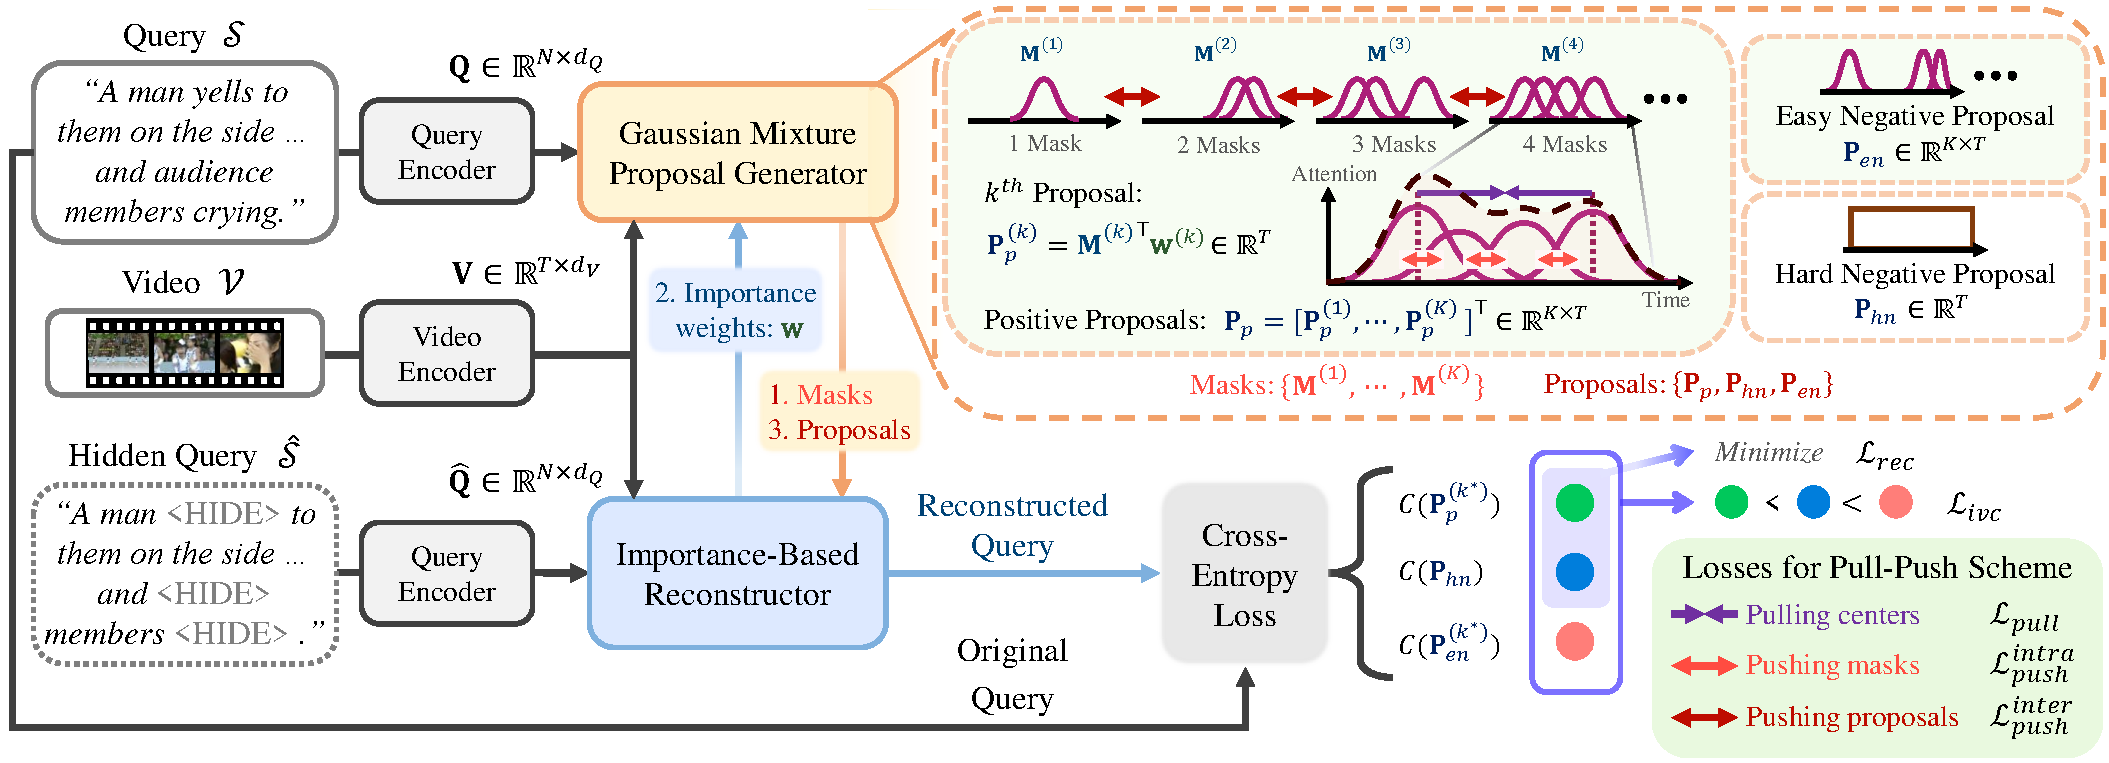
\includegraphics[width=\linewidth]{figures/1-framework.pdf}
  \caption{
  The overall scheme of the proposed method.
  % The proposal generator produces multiple Gaussian masks (positive, easy negative) and an entire video mask (hard negative) from the features representing both the video and sentence query.
  The Gaussian mixture proposal generator produces multiple Gaussian masks from the features representing both the video and sentence query.
  For the positive proposals, we define a Gaussian mixture proposal, where multiple Gaussian masks are combined via attentive pooling using the importance weights from the importance-based reconstructor.
  Further, to generate moderately coupled masks in the mixture proposal,
  we propose the pull-push learning scheme using $\mathcal{L}_{pull}$, $\mathcal{L}^{intra}_{push}$, and $\mathcal{L}^{inter}_{push}$.
  The importance-based reconstructor leverages the proposals to produce the reconstructed query from the hidden query. 
  % Our key contributions are highlighted with a green background.
  %For reconstruction, we minimize the cross-entropy losses of the positive proposals $\mathcal{L}_{rec}$.
  %To distinguish positive proposals from negative proposals, we perform contrastive learning with $\mathcal{L}_{ivc}$.
  }
\label{fig:framework}
\end{figure*}

% %% Fully supervised temporal video grounding %%%%%%%%%%%%%%%%%%%%%%%%%%%%%%
% \subsection{Fully supervised temporal video grounding}
% \label{sec:fully-supervised-temporal-video-grounding}
% %%%%%%%%%%%%%%%%%%%%%%%%%%%%%%%%%%%%%%%%%%%%%%%%%%%%%%%%
% % \textbf{Fully supervised temporal video grounding.}

% In fully supervised temporal video grounding, temporal locations of starting and ending times for every video-sentence pair are required during training.
% An early work~\cite{gao2017tall} makes sliding window-based proposals from a video and ranks the proposals according to the similarities between the proposal and the query.
% % Then, the proposal with the highest similarity is chosen as a predicted temporal location.
% % To make high-quality proposals, Xu \etal~\cite{xu2019multilevel} generate proposals guided by the query features to eliminate redundant proposals.
% % Also, Xiao \etal~\cite{xiao2021boundary} make high-quality proposals from an anchor-free model and use a visual-language fusion layer to model the multi-modal features.
% % To avoid heavy computations for generating proposals, proposal-free methods~\cite{ghosh2019excl, zeng2020dense} directly find temporal locations of starting and ending times without proposals.
% % Among the proposal-free methods, 
% The attention-based methods~\cite{yuan2019find, kim2021plrn} focus on specific video segments using a semantic phrase feature from the query.
% Similarly, multiple semantic phrases are leveraged for multi-level interaction between the query and video in \cite{mun2020local, kim2022swag}.
% However, the fully supervised methods require labor-intensive manual annotations of temporal locations which limit its scalability to real-world scenarios.
% Also, subjective annotations for temporal locations make trained models biased~\cite{yuan2021closer, zhou2021embracing}.
% Therefore, weakly supervised temporal video grounding has gained attention in recent years because it does not require temporal locations for video-sentence pairs.

%% Weakly supervised temporal video grounding %%%%%%%%%%%%%%%%%%%%%%%%%%%%%%
\subsection{Weakly Supervised Temporal Video Grounding}
\label{sec:weakly-supervised-temporal-video-grounding}
%%%%%%%%%%%%%%%%%%%%%%%%%%%%%%%%%%%%%%%%%%%%%%%%%%%%%%%%
% \textbf{Weakly supervised temporal video grounding.}

% In weakly supervised temporal video grounding, only video-sentence pairs are provided.

\paragraph{Sliding window-based methods}~\cite{huang2021cross, tan2021logan, mithun2019weakly, wang2021weakly, zhang2020counterfactual} generate proposals through the sliding window strategy and select the most probable proposal.
\cite{tan2021logan} proposes a multi-level co-attention model to learn visual-semantic representations.
\cite{huang2021cross} uses relations between sentences to understand cross-moment relations in videos.
However, sliding window-based methods make a lot of proposals with a predefined length and use Non-Maximum Suppression (NMS)~\cite{neubeck2006efficient} to reduce redundant proposals.
This process requires a large amount of computation. 
% and prior knowledge on the length distribution of temporal locations for each dataset.
The proposed method generates learnable Gaussian mixture proposals without using the sliding window.

\paragraph{Reconstruction-based methods}~\cite{lin2020weakly, zheng2022cnm, zheng2022cpl, song2020weakly, cao2023iterative} assume that well-generated proposals can reconstruct a sentence query from a randomly hidden sentence query.
Early works~\cite{lin2020weakly, song2020weakly} aggregate contextual information of video-sentence pairs to score proposals sampled at different scales.
However, these methods need to select one proposal from a large set of proposals, which requires heavy computation costs.
% song2020weakly is not sliding window-based
To solve this problem, other reconstruction-based methods~\cite{zheng2022cnm, zheng2022cpl} propose a learnable Gaussian proposal for a small set of proposals.
\cite{cao2023iterative} iteratively refines proposal confidence scores to prevent the grounding results from being biased.
Unlike the previous methods, our goal is to enhance the expression ability of proposals, hence we generate Gaussian mixture proposals which can effectively represent an arbitrary shape.
% and consider unmatched pairs of a sentence query and a video location inside the same video for contrastive learning.
% However, a Gaussian mask is a pre-determined shape with a high value on its center and lower values on its sides.
% Therefore, a single Gaussian mask is not suitable for expressing a temporal structure in a video because the temporal structure can be represented as an arbitrary shape with different importance according to the existence of semantic entities.


%% Gaussian Proposals in Video %%%%%%%%%%%%%%%%%%%%%%%
\subsection{Gaussian-based Approach}
\label{sec:gaussian-proposals-in-video}
%%%%%%%%%%%%%%%%%%%%%%%%%%%%%%%%%%%%%%%%%%%%%%%%%%%%%%%%

Gaussians have been studied in various tasks~\cite{zong2018deep, lee2018simple, piergiovanni2019temporal, long2019gaussian, zheng2022cnm, zheng2022cpl}.
For weakly-supervised temporal video grounding, \cite{zheng2022cnm, zheng2022cpl} propose learnable Gaussian proposals.
Specifically, \cite{zheng2022cnm} generates one Gaussian proposal for one temporal location, and \cite{zheng2022cpl} generates multiple Gaussian proposals and selects one proposal to predict a query-relevant temporal location.
% To depict an arbitrary shape of temporal structure, we make one Gaussian mixture proposal for one temporal location.
For action localization, 
\cite{long2019gaussian} uses multiple Gaussian proposals to localize multiple actions, where each single Gaussian proposal represents a temporal location of a specific action.
% Thus, the multiple Gaussian proposals do not work as a Gaussian mixture, which can not capture diverse events.

However, a single Gaussian is a pre-determined shape with a high value at its center, which is not suitable for expressing diverse query-relevant events.
To effectively represent the diverse events, we propose a Gaussian mixture proposal by learning importance, centroid, and range of every Gaussian in the mixture.
For action localization,
\cite{piergiovanni2019temporal} proposes a layer of Gaussian mixture that replaces a conventional convolutional layer to extract video features.
% Video features are applied to the Gaussian mixture layer to capture temporal information.
Also, there have been various tasks that train Gaussian mixture model in a feature space~\cite{zong2018deep, lee2018simple}.
Unlike these methods, we generate Gaussian mixture proposals that are directly implemented over a temporal location.
To represent a query-relevant temporal location that has diverse events, we propose a pull-push scheme to learn the moderately coupled Gaussian mixture.

